\subsection{Initialization and training}
After defining all the components of the network and their connections, we will explain how training is performed. The key idea behind the training process is to make the positions of the control points $P_i$ in the activation function learnable, allowing the model to adapt and learn any arbitrary shape for the activation function that best fits the data. \cite{KAN,kan_intro}

\subsubsection{Inizialization}
The only trainable part of a KAN network is the set of activation functions. In particular, for each activation function, we will train the weights $w_b$ and $w_s$ and the spline function $spline(x)$. 
\begin{itemize}
    \item We initialize the scaling factor for the spline function at 1: $w_s=1$. 
    \item Each spline function is initialized with $spline(x) \approx 0$.  This is done by drawing B-spline coefficients $c_i \sim \mathcal{N}(0, \sigma^2)$ with a small $\sigma$ around 0.1. It's likely used to ensure symmetry and stability in early training stages.
    \item We initialize the scaling factor for the residual connection function with the Xavier initialization as in MLPs: $w_b \sim \mathcal{U}\left[-\sqrt{\frac{6}{n_{\text{in}} + n_{\text{out}}}}, \sqrt{\frac{6}{n_{\text{in}} + n_{\text{out}}}}\right]$ where $n_{in}$ and $n_{out}$ are specific for any layers.
\end{itemize}

\subsubsection{Training}
Once the initialization has been defined, the KAN can be trained just like any other neural network. In particular for $N_{epochs}$ we will perform:
\begin{itemize}
    \item Forward propagation computing $KAN(\textbf{x}) = \boldsymbol{\Phi_{L-1}} \times \dots \times \boldsymbol{\Phi_{1}} \times \boldsymbol{\Phi_{0}} \times \textbf{x}$
    \item Backword propagation computing the loss with the LSM or the cross-entropy method and then adjusting $w_b$ and $ splines(x)$ with some method as GD, SGD, NM, BFGS, or others. The parameter $w_s$, which is a scale factor, will only be modified if the spline activation values evolve out of the fixed region during training.
\end{itemize}

\subsection{Hyperparameters and complexity}
The hyperparameters of a Kolmogorov-Arnold network are:
\begin{itemize}
    \item \textbf{L}: the depth of the KAN
    \item \textbf{N} $ \in \{\textbf{n}_0$, ... ,$\textbf{n}_l\}$: width of each layer
    \item \textbf{k}: each spline is a linear combination of k B-splines. Usually, k is very small for instance $k=3$.
    \item \textbf{G}: each B-splines has G control points
\end{itemize}

Then a KAN with hyperparameters \textbf{L},\textbf{N},\textbf{G},\textbf{k}, considering $N$ as the biggest $n_i \in N$, we will have in total $O(N^2L(G + k))  \simeq O(N^2LG)$ parameters. In contrast, an MLP with hyperparameters \textbf{L, N} needs only  $O(N^2L)$ parameters, which appears to be more efficient than KAN. Fortunately, KANs usually require much smaller N than MLPs, which not only saves parameters but also achieves better generalization and facilitates interpretability \cite{KAN}. 

\subsubsection{Performance (Accuracy)}
The most important Paper~\cite{KAN} has presented many performance-related results that compare the performance of KANs with MLP on various dummy/toy datasets. We will demonstrate that KANs are more effective when we want to perform non-linear regression or PDE solving.

In Figure~\ref{fig:re} the toy datasets are defined as follows:
\begin{enumerate}
    \item $f(x) = J_0(20x)$ (Bessel function): Represented by a $KAN(L=1,N=[1,1])$.
    \item $f(x, y) = e^{\sin(\pi x)+y^2}$: Represented by a $KAN(L=3,N=[2, 1, 1])$.
    \item $f(x, y) = xy$: Represented by a $KAN(L=3,N=[2, 2, 1])$.
    \item $f(x1_,\dots , x_{100}) = e^{\frac{1}{100} 
    \sum_{i=1}^{100} \sin^2(\frac{\pi x_i}{2})}$: Represented by a $KAN(L=3,N=[100, 1, 1])$.

    \item $f(x_1, x_2, x_3, x_4) = e^ {\sin(x_1^2 + x_2^2)+ \sin(x_3^2 + x_4^2)}$ : Represented by a $KAN(L=3,N=[4,4, 2, 1])$.
\end{enumerate}

We train these KANs by increasing grid points every 200 steps, in total covering

$G =\{3, 5, 10, 20, 50, 100, 200, 500, 1000\}$. We train MLPs with different depths and widths as baselines. Both MLPs and KANs are trained with LBFGS for 1800 steps in total.


\begin{figure}[H]
    \centering
    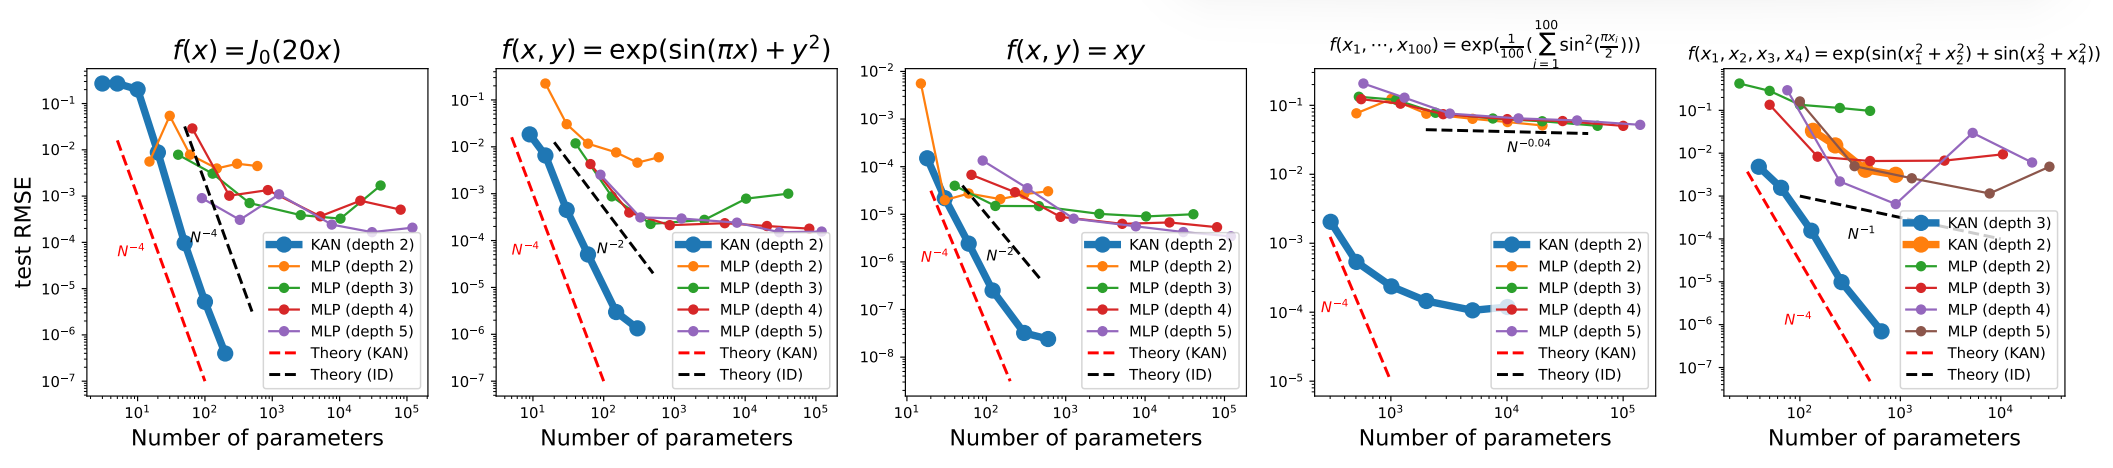
\includegraphics[width=0.95\linewidth]{Images/result.png}
    \caption{Results for KAN with toy dataset}
    \label{fig:re}
\end{figure}

In all the plots we can see that
\begin{itemize}
    \item KANs consistently outperform MLPs, achieving significantly lower test loss across a range of parameters, and at much lower network depth (number of layers).
    \item KANs demonstrate superior efficiency, with steeper declines in loss, particularly noticeable with fewer parameters.
    \item MLP's performance almost stagnates with increasing the number of parameters.
    \item The theoretical lines $N^{-4}$ for KAN and $N^{-2}$ for ideal models (ID), show that KANs closely follow their expected theoretical performance.
\end{itemize}

\subsubsection{Drawbacks}
Currently, the biggest bottleneck of KANs lies in their slow training. KANs are typically 10 times slower than MLPs, given the same number of parameters (though KANs require fewer parameters than MLPs to accomplish the same task). This is primarily caused by the complex reshaping of $\text{spline}(x)$, particularly on B-spline control points.

We should be honest that the first paper on KANs was pre-released in June 2024 \cite{KAN}, so at this point, no one is focused on optimization. This issue will likely be addressed as an engineering problem to be improved in the future rather than a fundamental limitation.

If one wants to train a model quickly, MLPs should be used. In other cases, however, KANs can be comparable to or even better than MLPs. The decision tree in Figure~\ref{fig:dtree} can assist in determining when to use a KAN. In summary, if you value interpretability and/or accuracy and slow training is not a major concern, we suggest trying KANs.

\begin{figure}[H]
    \centering
    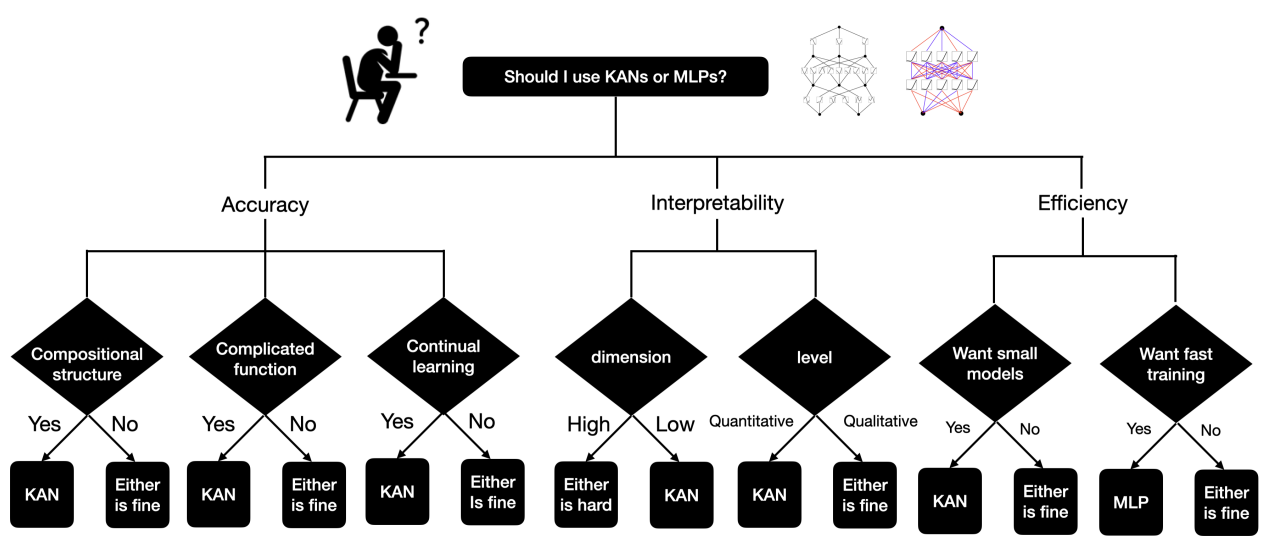
\includegraphics[width=0.75\linewidth]{LATEX//Images/MLP_KAN.png}
    \caption{MLP vs KAN: decision tree}
    \label{fig:dtree}
\end{figure}